\section*{ÔN TẬP KIỂM TRA CUỐI KÌ 1 - ĐỀ 02}
\setcounter{ex}{0}\setcounter{bt}{0}
\noindent{\bf\fontfamily{qag}\selectfont\color{violet}A. PHẦN TRẮC NGHIỆM}
\Opensolutionfile{ans}[ans/ansBTTeX2]

\begin{ex}%[06]%[Nguyễn Diệu Linh]%[0D1Y1-3]
Mệnh đề phủ định của mệnh đề $P(x):$ $``x^2+3x+1>0$ với mọi $x"$ là
\choice
{Tồn tại $x$ sao cho $x^2+3x+1>0$}
{\True Tồn tại $x$ sao cho $x^2+3x+1\le 0$}
{Tồn tại $x$ sao cho $x^2+3x+1=0$ 	}
{Tồn tại $x$ sao cho $x^2+3x+1<0$}
\loigiai
{
Phủ định của mệnh đề $P(x)$ là $\overline{P(x)}$ : $``$Tồn tại $x$ sao cho $x^2+3x+1\le 0"$.
}
\end{ex}

\begin{ex}%[02]%[Nguyễn Diệu Linh]%[0D1B1-4]
Trong các câu sau, câu nào là mệnh đề \textbf{đúng}?
\choice
{Nếu $a\ge b$ thì $a^2\ge b^2$}
{\True Nếu $a$ chia hết cho $9$ thì $a$ chia hết cho $3$}
{Nếu em chăm chỉ thì em thành công}
{Nếu một tam giác có một góc bằng $60^\circ $ thì tam giác đó đều}
\loigiai
{
\begin{itemize}
\item Mệnh đề $``$Nếu $a\ge b$ thì $a^2\ge b^2"$ là một mệnh đề sai vì $b\le a < 0$ thì $a^2\le b^2$ .
\item Mệnh đề $``$Nếu $a$ chia hết cho $9$ thì $a$ chia hết cho $3"$ là mệnh đề đúng.\\
Vì $a$ $\vdots$ $9\Rightarrow \heva{&a=9n, n\in \mathbb{Z}\\&9\hspace{0.15cm}\vdots\hspace{0.15cm} 3}\Rightarrow a$ $\vdots$  $3$.
\item $``$Nếu em chăm chỉ thì em thành công$"$ chưa là mệnh đề vì chưa khẳng định được tính đúng, sai.
\item Mệnh đề $``$Nếu một tam giác có một góc bằng $60^\circ $ thì tam giác đó đều$"$ là mệnh đề sai vì chưa đủ điều kiện để khẳng định một tam giác là đều.
\end{itemize}
}
\end{ex}

\begin{ex} %[0D1Y2-2]
Cho $A$ là một tập hợp. Trong các mệnh đề sau, mệnh đề nào \textbf{đúng}?
\choice
{$A\in A$}
{$\varnothing \in A$}
{\True $A \subset A$}
{$A \notin \{A\}$}
\loigiai{
Mệnh đề đúng là $A \subset A$ vì theo tính chất $A\subset A, \forall A$.
}
\end{ex}

\begin{ex}%[Đỗ Đường Hiếu - ĐCHT THPT]%[0D1B3-2]
Cho tập hợp $ A=\left\{-1;0;1;2;3\right\}$ và $B=\left\{-1;1;3;4;5\right\}$. Mệnh đề nào sau đây là \textbf{sai}?
\choice
{$A\cap B=\left\{-1;1;3\right\}$}
{$B\setminus A=\left\{4;5\right\}$}
{$A\cup B=\left\{-1;0;1;2;3;4;5\right\}$}
{\True $A\setminus B=\left\{0;3\right\}$}
\loigiai{
Ta có $0;2\in A$ và $ 0;2\notin B\Rightarrow A\setminus B=\left\{0;2\right\}$.\\
Do đó, mênh đề sai là \lq\lq$A\setminus B=\left\{0;3\right\}$\rq\rq.
}
\end{ex}

\begin{ex}%[Lê Quốc Dũng-Dự Án TEX TLDH5]%[0D1K3-3]
Một lớp có $45$ học sinh. Mỗi em đều đăng ký chơi ít nhất một trong hai môn: bóng đá và bóng chuyền. Có $35$ em đăng ký môn bóng đá, $15$ em đăng ký môn bóng chuyền. Hỏi có bao nhiêu em đăng ký chơi cả $2$ môn?
\choice
{\True $5$}
{$10$}
{$30$}
{$25$}
\loigiai{
\immini{Gọi A là tập hợp các học sinh đăng ký chơi bóng đá, B là tập hợp các học sinh đăng ký chơi bóng chuyền. Dựa vào biểu đồ Ven, ta có số học sinh đăng ký cả 2 môn là \[\left|A\cap B\right|=\left| A\right|+\left| B\right|-\left|A\cup B\right|=35+15-45=5.\]
}{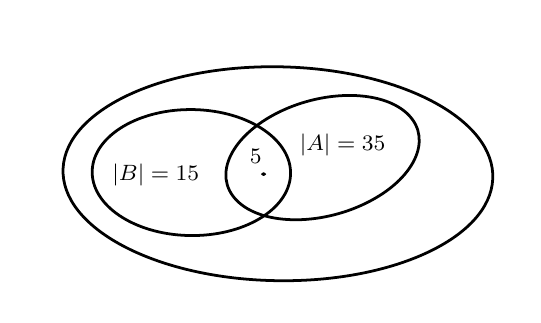
\begin{tikzpicture}[xscale=0.7,yscale=0.5, font=\footnotesize, line join=round, line cap=round, >=stealth]
\clip(1.64,-2.56) rectangle (10.44,4.22);
\draw [rotate around={-2:(6.18,0.51)},line width=1pt] (6.18,0.51) ellipse (3.9cm and 2.716cm);
\draw [rotate around={-2:(4.61,0.54)},line width=1pt] (4.61,0.54) ellipse (1.8cm and 1.6cm);
\draw [rotate around={34.66:(6.99,0.92)},line width=1pt] (6.99,0.92) ellipse (1.9cm and 1.4cm);
\draw (6.4,1.78) node[anchor=north west] {$|A|=35$};
\draw (3,1.02) node[anchor=north west] {$|B|=15$};
\draw (5.78,0.96) node{$5$};
\begin{scriptsize}
\draw [fill=black] (5.92,0.5) circle (1pt);
\end{scriptsize}
\end{tikzpicture}}
}
\end{ex}

\begin{ex}%[VanLo HoaTrung, du an tex hoa tai lieu 10]%[0D4Y4-1]
Cho bất phương trình $2x+3y \le 0$ $(1)$. Chọn khẳng định đúng trong các khẳng định sau
\choice
{Bất phương trình $(1)$ chỉ có một nghiệm duy nhất}
{Bất phương trình $(1)$ vô nghiệm}
{\True Bất phương trình $(1)$ luôn có vô số nghiệm}
{Bất phương trình  có tập nghiệm là $\mathbb{R}$}
\loigiai{
Bất phương trình $2x+3y-6\le0$. có miền nghiệm phần tô màu kể cả bờ là đường thẳng $2x+3y-6=0$.\\
Vậy bất phương trình vô số nghiệm.
}
\end{ex}

\begin{ex}%[0D4Y4-4]
Miền nghiệm của hệ bất phương trình $\heva{&2x-5y-1>0\\&2x+y+5>0\\&x+y+1<0}$ chứa điểm nào trong các điểm sau?
\choice
{$(0;0)$}
{$(1;0)$}
{\True $(0;-2)$}
{$(0;2)$}
\loigiai{Thay điểm $(0;-2)$ vào hệ bất phương trình, ta có
$\heva{&2 \cdot 0 - 5 \cdot (-2)-1=9>0\\&2 \cdot 0 + (-2) +5=3>0\\&0+(-2)+1=-1<0}$ (đúng).
}
\end{ex}

\begin{ex}%[Dự án Tex Khối 10-11 W-T-Begin lần 4]%[Biên soạn: Tuan Nguyen, Phản biện: Phan Văn Thành]%[0D4B4-1]
Trong các cặp số sau đây, cặp nào \textbf{không} là nghiệm của bất phương trình $x-4y+1 \geq 0$?
\choice
{$(-1;0)$}
{$(-2;-1)$}
{\True $(-1;3)$}
{$(0;0)$}
\loigiai{
Ta có $(-1)-4\cdot 3+1\ge 0$ là mệnh đề sai nên cặp số $(-1;3)$ không là nghiệm của của bất phương trình trên.
}
\end{ex}

\begin{ex}%[0D4B4-4]
Điểm nào sau đây thuộc miền nghiệm của hệ bất phương trình $\heva{& 2x+3y-1>0\\& 5x-y+4<0.}$
\choice
{$(0;0)$}
{$(-2;0)$}
{$(-1;-4)$}
{\True $(-3;4)$}
\loigiai{
Thay tọa độ từng điểm vào mỗi hệ bất phương trình.
\begin{itemize}
\item Với điểm $(0;0)$ ta được $2\cdot 0+3 \cdot 0-1=-1<0$ (sai) nên không thỏa mãn bất phương trình đầu.
\item Với điểm $(-2;0)$ ta được $2 \cdot (-2)+3\cdot 0-1=-5<0$ (sai) nên không thỏa mãn bất phương trình đầu.
\item Với điểm $(-1;-4)$ ta được $2 \cdot (-1)+3 \cdot (-4)-1=-15<0$ (sai) nên không thỏa mãn bất phương trình đầu.
\item Với điểm $(-3;4)$ ta được $\heva{&2 \cdot(-3)+3\cdot 4-1=5>0 \\ &5 \cdot (-3)-4+4=-15<0}$ (đúng) thỏa mãn cả hai bất phương trình của hệ.
\end{itemize}
}
\end{ex}

\begin{ex}%[0D2B1-1]
Cho họ đường thẳng $d_{m}:(m+1)x-2(m-2)y+3=0$ và các mệnh đề
\begin{enumerate}
\item $d_{m}$ luôn đi qua hai điểm cố định.
\item $d_{1}\parallel d_{5}$.
\item $d_{1}\perp d_{3}$.
\item $d_{5}$ là đường phân giác thứ nhất của hệ trục tọa độ $Oxy$.
\end{enumerate}
Tìm mệnh đề \textbf{sai} trong các mệnh đề trên.
\choice
{1}
{1, 3}
{2, 3}
{\True 1,2,3,4}
\loigiai{
\begin{enumerate}
\item Gọi $(x_{0};y_{0})$ là điểm cố định của họ $d_{m}$. Ta có\\
$m(x_{0}-2y_{0})+(x_{0}+4y_{0}+3)=0$, $\forall m\Leftrightarrow\heva{
&x_{0}-2y_{0}=0\\
&x_{0}+4y_{0}+3=0
}\Leftrightarrow\heva{
&x_{0}=-1\\
&y_{0}=-\dfrac{1}{2}
}$
\item $d_{1}\colon 2x+2y+3=0$ và $d_{5}\colon 6x-6y+3=0\Rightarrow d_{1}$ không song song với $ d_{5}$.
\item $d_{1}\colon 2x+2y+3=0$ và $d_{3}\colon 4x-2y+3=0\Rightarrow d_{1}$ cắt $ d_{3}$ và không vuông góc.
\item $d_{5}\colon 6x-6y+3=0\Rightarrow$ $d_{5}$ không phải là phân giác thứ nhất của hệ tọa độ $Oxy$.
\end{enumerate} }
\end{ex}

\begin{ex}%[0D2B1-2]%[Lê Văn Vĩ, Dự án TLDH5]% Cau 42.
Cho hàm số $ y=\dfrac{x+2}{\sqrt{x-1}}+\sqrt{3-x}$. Tập xác định của hàm số này là?
\choice
{\True $\mathscr{D}=\left[ 1;3 \right]$}
{$\mathscr{D}=\left( 1;3 \right]$}
{$\mathscr{D}=\left( -\infty ;3 \right]$}
{$\mathscr{D}=\left( 1;+\infty \right)$}
\loigiai{
Hàm số xác định khi và chỉ khi $\heva{& x-1>0 \\
& 3-x\ge 0}\Leftrightarrow 1<x\le 3$.}
\end{ex}

\begin{ex}%[0D2B1-3]
Xét tính đồng biến, nghịch biến của hàm số $f(x)=\dfrac{x-3}{x+5}$ trên khoảng $(-\infty ;-5)$ và trên khoảng $(-5;+\infty)$. Khẳng định nào sau đây \textbf{đúng}?
\choice
{Hàm số nghịch biến trên $(-\infty ;-5)$, đồng biến trên $(-5;+\infty)$}
{Hàm số đồng biến trên $(-\infty ;-5)$, nghịch biến trên $(-5;+\infty)$}
{Hàm số nghịch biến trên các khoảng $(-\infty ;-5)$ và $(-5;+\infty)$}
{\True Hàm số đồng biến trên các khoảng $(-\infty ;-5)$ và $(-5;+\infty)$}
\loigiai{
Ta có\\ $f\left(x_1\right)-f\left(x_2\right)=\left(\dfrac{x_1-3}{x_1+5}\right)-\left(\dfrac{x_2-3}{x_2+5}\right)=\dfrac{\left(x_1-3\right)\left(x_2+5\right)-\left(x_2-3\right)\left(x_1+5\right)}{\left(x_1+5\right)\left(x_2+5\right)}=\dfrac{8\left(x_1-x_2\right)}{\left(x_1+5\right)\left(x_2+5\right)}$.\\
Xét $k=\dfrac{f\left(x_1\right)-f\left(x_2\right)}{x_1-x_2}=\dfrac 8{\left(x_1+5\right)\left(x_2+5\right)}$ $(x_1 \neq x_2)$.
\begin{itemize}
\item Với mọi $x_1, x_2\in(-\infty ;-5)$ , ta có $x_1+5<0$ và $x_2+5<0$, suy ra $k>0$, do đó hàm số đồng biến trên $(-\infty ;-5)$.
\item Với mọi $x_1, x_2\in(-5;+\infty)$, ta có $x_1+5>0$ và $x_2+5>0$, suy ra $k>0$, do đó hàm số đồng biến trên $(-5;+\infty)$.
\end{itemize}
}
\end{ex}

\begin{ex}%[0D2Y3-1]%[Trần Ngọc Phú - Dự án TLDH5]
\immini{Tìm hàm số bậc hai có bảng biến thiên như hình vẽ bên.
\choice
{\True $y=x^2-4x+5$}
{$y=x^2-2x+1$}
{$y=-x^2+4x-3$}
{$y=x^2-4x-5$}}
{
\begin{tikzpicture}
\tkzTabInit[nocadre=false,lgt=1,espcl=2.5,deltacl=0.6]
{$x$ /0.6, $y$ /1.5}
{$-\infty$,$2$,$+\infty$}
\tkzTabVar{+/$+\infty$,-/$1$,+/$+\infty$}
\end{tikzpicture}
}
\loigiai{
Dựa vào bảng biến thiên ta có $a > 0$ và hàm số có tọa độ đỉnh là $(2;1)$.\\Vậy hàm số $y=x^2-4x+5$ thỏa bảng biên thiên.
}
\end{ex}

\begin{ex}%[0D2Y3-3]%[Trần Ngọc Phú - Dự án TLDH5]
Cho parabol $\left( P\right) $ có phương trình $y=x^2-2x+4$. Tìm điểm mà parabol đi qua.
\choice
{$P(4;0)$}
{$N(-3;1)$}
{$M(-3;19)$}
{\True $Q(2;4)$}
\loigiai{Lần lượt thay tọa độ các điểm $P$, $N$, $M$, $Q$ vào phương trình $y=x^2-2x+4$.\\ Dễ thấy $Q(2;4)$ thỏa phương trình.
}
\end{ex}

\begin{ex}%[0D2B3-1]%[Lê Văn Vĩ, Dự án TLDH5] Cau 39.
Hàm số $ y=2x^2+4x-1$ đồng biến trên khoảng nào sau đây?
\choice
{$\left( -\infty ;-2 \right)$}
{$\left( -2;2 \right)$}
{\True $\left( -1;+\infty \right)$}
{$\left( -\infty ;+\infty \right)$}
\loigiai{
$ y=2x^2+4x-1$ có tọa độ đỉnh là $I\left( -1;-3 \right)$.
\begin{center}
\begin{tikzpicture}[scale=1, font=\footnotesize, line join=round, line cap=round, >=stealth]
\tkzTabInit [lgt=1.2,espcl=2.5,deltacl=0.6]{$x$/0.6,  $y$/1.5}
{$-\infty$, $-1$,$+\infty$}
\path
(N11)node[below](A){$+\infty$}
(N22)node[above](B){$-3$}
(N31)node[below](C){$+\infty$};
\foreach \x/\y in {A/B,B/C} \draw[->] (\x)--(\y);
\end{tikzpicture}
\end{center}
Hàm số $y=2x^2+4x-1$ đồng biến trên khoảng $\left( -1;+\infty \right)$.}
\end{ex}

\begin{ex}%[0D4Y5-1]
Biểu thức nào sau đây là tam thức bậc hai?
\choice
{$f(x)=-2 x+1$}
{$f(x)=x^3-3 x+5$}
{\True $f(x)=2 x^2-5 x+2$}
{$f(x)=a x^2+b x+c$}
\loigiai{
Theo định nghĩa thì $f(x)=2 x^2-5 x+2$ là tam thức bậc hai
}
\end{ex}

\begin{ex}%[Đoàn Minh Tân]%[0D4Y5-1]
Tam thức $f(x)=x^2-12x-13$ nhận giá trị âm khi và chỉ khi
\choice
{$x<-13$ hoặc $x>1$}
{$x<-1$ hoặc $x>13$}
{$-13<x<1$}
{\True $-1<x<13$}
\loigiai{
Tam thức $f(x)=x^2-12x-13$ có $\Delta =196>0$, hai nghiệm $x_1=-1$, $x_2=13$ và hệ số $a=1>0$.\\
Bảng xét dấu của $f(x)$ như sau
\begin{center}

\begin{tikzpicture}
\tkzTabInit[nocadre=false, lgt=1.5, espcl=1.5]
{$x$ /0.6,$f(x)$ /0.6}
{$-\infty$,$-1$,$13$, $+\infty$}
\tkzTabLine{,+,0,-,0,+}
\end{tikzpicture}
\end{center}
Do đó $f(x)<0$ khi $-1<x<13$.
}
\end{ex}

\begin{ex}%[0D4B5-2]
Cho tam thức bậc hai $f(x)=-x^2-4x+5$. Tìm tất cả giá trị của $x$ để $f(x)\geqslant 0$.
\choice
{$x\in (-\infty;-1]\cup [5;+\infty)$}
{$x\in [-1;5]$}
{\True $x\in [-5;1]$}
{$x\in (-5;1)$}
\loigiai{
Ta có $f(x)=0$ $ \Leftrightarrow $ $-x^2-4x+5=0$ $ \Leftrightarrow $ $x=1$, $x=-5$.\\
Mà hệ số $a=-1<0$ nên: $f(x)\geqslant 0$ $ \Leftrightarrow $ $x\in [-5;1]$.}
\end{ex}

\begin{ex}%[0D3B2-4]
Nghiệm của phương trình $x-\sqrt{3x^2-9x+1}=2$ là
\choice
{\True $x=3$}
{$x=-\dfrac{1}{2}$}
{$\hoac{&x=-\dfrac{1}{2}\\&x=3}$}
{$x\in\varnothing$}
\loigiai{Phương trình đã cho được viết lại $\sqrt{3x^2-9x+1}=x-2$.\\
Bình phương hai vế của phương trình trên, ta được
\begin{eqnarray*}
3x^2-9x+1=(x-2)^2\Rightarrow 3x^2-9x+1=x^2-4x+4\Rightarrow 2x^2-5x-3=0\Rightarrow x=3 \ \text{hoặc} \ x=-\dfrac{1}{2}.
\end{eqnarray*}
Thay lần lượt các giá trị trên vào phương trình đã cho, ta thấy $x=3$ thỏa mãn.\\
Vậy nghiệm của phương trình đã cho là $x=3$.
}
\end{ex}

\begin{ex}%[0D3B2-4]
Biết $\alpha$ là nghiệm của phương trình $\sqrt{2x^2-4x-1}=2-x$. Chọn khẳng định đúng.
\choice
{$2<\alpha<3$}
{$-2<\alpha<2$}
{$\alpha^2>5$}
{\True $-3<\alpha<-2$}
\loigiai{
Trước hết ta giải bất phương trình $2-x\geq 0\Leftrightarrow x\leq 2.\; (*)$
\allowdisplaybreaks
\begin{eqnarray*}
&&\sqrt{2x^2-4x-1}=2-x=2-x\\
&\Rightarrow&2x^2-4x-1=(2-x)^2\\
&\Rightarrow&x^2=5\\
&\Rightarrow&\hoac{&x=-\sqrt{5}\\&x=\sqrt{5}.}
\end{eqnarray*}
Trong hai giá trị trên, chỉ có $x=-\sqrt{5}$ thỏa mãn $(*)$.\\
Vậy phương trình đã cho có một nghiệm $x=-\sqrt{5}$.
}
\end{ex}

\begin{ex}%[0D3B2-4]
Số nghiệm của phương trình	$\sqrt{x^2-5x+2}=\sqrt{-x-1}$ là
\choice
{\True 0}
{1}
{2}
{4}
\loigiai{\begin{eqnarray*} \sqrt{x^2-5x+2}=\sqrt{-x-1}
&\Rightarrow & x^2-5x+2 = -x-1\\
& \Rightarrow & x^2 -4x+3= 0\\
& \Rightarrow & \hoac{& x=1  \\& x=3.}
\end{eqnarray*}
Các nghiệm không thỏa mãn phương trình ban đầu. \\ Vậy phương trình có tập nghiệm $S =\varnothing $.}
\end{ex}

\begin{ex}%[0H2Y1-1]
Cho $\alpha$ là góc tù. Khẳng định nào sau đây \textbf{đúng}?
\choice
{$\sin \alpha<0$}
{$\cos \alpha>0$}
{\True $\tan \alpha<0$}
{$\cot \alpha>0$}
\loigiai{
Do $\alpha$ là góc tù nên $\sin\alpha>0$, $\cos\alpha<0$, $\tan\alpha<0$ và $\cot\alpha<0$.
}
\end{ex}

\begin{ex}%[0H2Y3-1]
Chọn công thức đúng trong các đáp án sau
\choice
{$S=\dfrac{1}{2}bc\sin B$}
{\True $S=\dfrac{1}{2}bc\sin A$}
{$S=\dfrac{1}{2}ab\sin B$}
{$S=\dfrac{1}{2}ac\sin A$}
\loigiai{
Công thức đúng là $S=\dfrac{1}{2}bc\sin A$.
}
\end{ex}

\begin{ex}%[0H2Y3-1]
Tam giác $ ABC$ có $ AB=5$, $BC=7$, $CA=8$. Số đo góc $ \widehat{A}$ bằng
\choice
{$ 90^\circ $}
{$ 45^\circ $}
{\True $ 60^\circ $}
{$ 30^\circ $}
\loigiai
{Theo định lí hàm cosine, ta có $ \cos{A}=\dfrac{AB^2+AC^2-BC^2}{2AB\cdot AC}=\dfrac{5^2+8^2-7^2}{2\cdot 5\cdot 8}=\dfrac{1}{2}$.\\
Do đó, $ \widehat{A}=60^\circ $.}
\end{ex}

\begin{ex}%[0H2B1-2]
Cho biết $\tan \alpha =-3$. Giá trị của $P=\dfrac{6\sin \alpha -7\cos \alpha }{6\cos \alpha +7\sin \alpha }$ bằng bao nhiêu?
\choice
{$P=\dfrac{4}{3}$}
{\True $P=\dfrac{5}{3}$}
{$P=-\dfrac{4}{3}$}
{$P=-\dfrac{5}{3}$}
\loigiai
{Ta có $P=\dfrac{6\sin \alpha -7\cos \alpha }{6\cos \alpha +7\sin \alpha }=\dfrac{6\dfrac{\sin \alpha }{\cos \alpha }-7}{6+7\dfrac{\sin \alpha }{\cos \alpha }}=\dfrac{6\tan \alpha -7}{6+7\tan \alpha }=\dfrac{5}{3}$.}
\end{ex}

\begin{ex}%[0H1Y1-1]
Chọn khẳng định đúng trong các khẳng định sau.
\choice
{vectơ là một đường thẳng có hướng}
{vectơ là một đoạn thẳng}
{\True vectơ là một đoạn thẳng có hướng}
{vectơ là một đoạn thẳng không phân biệt điểm đầu và điểm cuối}
\loigiai{vectơ là một đoạn thẳng có hướng.
}
\end{ex}

\begin{ex}%[Lê Minh Thiện Anh, Dự án BG10-Lần2]%[0H1Y1-3]
Hai véc-tơ được gọi là bằng nhau khi và chỉ khi
\choice
{Giá của chúng trùng nhau và độ dài của chúng bằng nhau}
{Chúng trùng với một trong các cặp cạnh đối của hình bình hành}
{Chúng trùng với một trong các cặp cạnh của tam giác đều}
{\True Chúng cùng hướng và có độ dài bằng nhau}
\loigiai
{Theo định nghĩa hai véc-tơ bằng nhau là hai véc-tơ có cùng hướng và độ dài bằng nhau.}
\end{ex}

\begin{ex}%[Dự án Tex hóa Tài Liệu 10 Mới - Lê Văn Hiếu]%[0H1B1-1]
Cho tứ giác $ABCD$. Có bao nhiêu vectơ khác vectơ - không có điểm đầu và điểm cuối là các đỉnh của tứ giác?
\choice
{$4$}
{$6$}
{$8$}
{\True $12$}
\loigiai{
Số vectơ cần tìm là: $4\cdot3=12$.}
\end{ex}

\begin{ex}%[Lê Minh Thiện Anh, Dự án BG10-Lần2]%[0H1Y2-1]
Cho ba điểm $A$, $B$, $C$ phân biệt. Đẳng thức nào sau đây là đẳng thức \textbf{sai}?
\choice
{$\overrightarrow{AB}+\overrightarrow{BC}=\overrightarrow{AC}$}
{\True $\overrightarrow{CA}+\overrightarrow{AB}=\overrightarrow{BC}$}
{$\overrightarrow{BA}+\overrightarrow{AC}=\overrightarrow{BC}$}
{$\overrightarrow{AB}-\overrightarrow{AC}=\overrightarrow{CB}$}
\loigiai{
Theo quy tắc cộng cho $3$ điểm, ta có $\overrightarrow{CA}+\overrightarrow{AB}=\overrightarrow{CB}$.
}
\end{ex}

\begin{ex}%[Trần Quốc, BG10-2022, Nhóm 9]%[0H1Y3-1]
	Cho điểm $B$ nằm giữa hai điểm $A$ và $C$, với $AB=2a$, $AC=6a$. Đẳng thức nào dưới đây là đẳng thức đúng?
	\choice
	{\True $\overrightarrow{B C}=-2 \overrightarrow{B A}$}
	{$\overrightarrow{B C}=4 \overrightarrow{A B}$}
	{$\overrightarrow{B C}=-2 \overrightarrow{A B}$}
	{$\overrightarrow{B C}=-4 \overrightarrow{A B}$}
	\loigiai{
		\immini{
			Theo giả thiết ta có $BC=AC-AB=4a$. \\
			Vì $\overrightarrow{BA}$ và $\overrightarrow{BC}$ ngược hướng nên  $\overrightarrow{B C}=-2 \overrightarrow{B A}$.
		}{
			\begin{tikzpicture}[font=\footnotesize,line join=round, line cap=round, >=stealth,scale=1]
				\coordinate (A) at (0,0);
				\coordinate (C) at (6,0);
				\coordinate (B) at (2,0);
				\draw (A)--(C);
				\foreach \x/\pos in {A/180, B/90, C/0} \fill (\x) circle(1pt) node[{shift=(\pos:0.25)}]{$\x$};
				\foreach \x in {1,3,4,5} \fill (\x,0) circle(1pt);
			\end{tikzpicture}
		}
	}
\end{ex}

\begin{ex}%[Trần Quốc, BG10-2022, Nhóm 9]%[0H1B3-1]
Cho tam giác $ABC$ đều cạnh $a$. Khi đó, giá trị $\left| \overrightarrow{AB}+\overrightarrow{AC}\right|$ bằng
\choice
{\True $a \sqrt{3}$}
{$\dfrac{a \sqrt{3}}{2}$}
{$2a$}
{$\dfrac{a \sqrt{3}}{3}$}
\loigiai{
\immini{
Gọi $M$ là trung điểm của $BC$. \\
Vì $AM$ là đường trung tuyến của tam giác đều nên \[AM=\dfrac{\sqrt{3}}{2}\cdot a=\dfrac{a\sqrt{3}}{2}.\]
Khi đó, ta có
\[\left| \overrightarrow{AB}+\overrightarrow{AC}\right| = \left|2\overrightarrow{AM} \right| = 2\cdot AM = 2\cdot \dfrac{a\sqrt{3}}{2} = a\sqrt{3}.\]
}{
\begin{tikzpicture}[line cap=round,line join=round,>=stealth,scale=0.9,font=\footnotesize]
\coordinate (B) at (0,0);
\coordinate (C) at (4,0);
\coordinate (A) at (2,3.46);
\coordinate (M) at ($(B)!.5!(C)$);
\draw (A)--(B)--(C)--(A)--(M);
\foreach \x/\pos in {A/90, B/180, C/0, M/-90} \fill (\x) circle(1pt) node[{shift=(\pos:0.25)}]{$\x$};
\end{tikzpicture}
}
}
\end{ex}

\begin{ex}%[0H1B3-2]
Cho tam giác $ ABC $  có trọng tâm $ G $ và $ M $, $ N $, $ P $ lần lượt là trung điểm của các đoạn thẳng $ BC $, $ CA $, $ AB $. Khẳng định nào sau đây là \textbf{sai}?
\choice
{$ \overrightarrow{AM}+\overrightarrow{BN}+\overrightarrow{CP}=\vec{0} $}
{$ \overrightarrow{GM}+\overrightarrow{GN}+\overrightarrow{GP}=\vec{0} $}
{\True $ \overrightarrow{GC}-2\overrightarrow{GP}=\vec{0} $}
{$ \overrightarrow{AG}+\overrightarrow{BG}+\overrightarrow{CG}=\vec{0} $}
\loigiai{
\begin{center}
\begin{tikzpicture}[>=latex,line join=round,line cap=round,font=\footnotesize,scale=0.85,line width=1pt]
\coordinate[label=above:$A$](A) at (0,0);
\coordinate[shift=(-130:3.5cm),label=below:$B$] (B) at (0,0);
\coordinate[shift=(-30:4cm),label=below:$C$] (C) at (0,0);
\coordinate[label=below:$M$](M) at ($ (B)!0.5!(C) $);
\coordinate[label=right:$N$](N) at ($ (A)!0.5!(C) $);
\coordinate[label=left:$P$](P) at ($ (A)!0.5!(B) $);
\coordinate[label=above right:$G$](G) at ($ (A)!2/3!(M) $);
\draw (A)--(B)--(C)--(A) (A)--(M) (B)--(N) (C)--(P);
\foreach \toado in {A,B,C,M,N,P,G}
{
\fill (\toado) circle (1.5pt);
}
\end{tikzpicture}
\end{center}
Xét đẳng thức $ \overrightarrow{AM}+\overrightarrow{BN}+\overrightarrow{CP}=\vec{0} $.\\
Ta có: $\overrightarrow{AM}+\overrightarrow{BN}+\overrightarrow{CP}=\dfrac{2}{3}\overrightarrow{AG} + \dfrac{2}{3}\overrightarrow{BG}+\dfrac{2}{3}\overrightarrow{CG}=-\dfrac{2}{3}\left( \overrightarrow{GA}+ \overrightarrow{GB}+ \overrightarrow{GC}\right)=\vec{0} $.\\
Vậy $ \overrightarrow{AM}+\overrightarrow{BN}+\overrightarrow{CP}=\vec{0} $ đúng.\\
Xét đẳng thức $ \overrightarrow{GM}+\overrightarrow{GN}+\overrightarrow{GP}=\vec{0} $.\\
Ta có: $ \overrightarrow{GM}+\overrightarrow{GN}+\overrightarrow{GP}=-\dfrac{1}{2}\left(\overrightarrow{GA}+ \overrightarrow{GB}+ \overrightarrow{GC} \right) =\vec{0}$.\\
Vậy $ \overrightarrow{GM}+\overrightarrow{GN}+\overrightarrow{GP}=\vec{0} $ đúng.\\
Xét đẳng thức $ \overrightarrow{GC}-2\overrightarrow{GP}=\vec{0} $.\\
$ \overrightarrow{GC}-2\overrightarrow{GP}=\vec{0} \Rightarrow \overrightarrow{GC}=2\overrightarrow{GP}\; \; (\text{sai})$.\\
Vậy $ \overrightarrow{GC}-2\overrightarrow{GP}=\vec{0} $ (sai).\\
Xét đẳng thức $ \overrightarrow{AG}+\overrightarrow{BG}+\overrightarrow{CG}=\vec{0} $.\\
Ta có: $ \overrightarrow{AG}+\overrightarrow{BG}+\overrightarrow{CG}=-\left(\overrightarrow{GA}+ \overrightarrow{GB}+ \overrightarrow{GC} \right) =\vec{0} $.\\
Vậy $ \overrightarrow{AG}+\overrightarrow{BG}+\overrightarrow{CG}=\vec{0} $ đúng.
}
\end{ex}

\begin{ex}%[0H2Y2-1]
Cho hai véc-tơ $\overrightarrow{a}$ và $\overrightarrow{b}$ thỏa mãn $\left|\overrightarrow{a}\right|=\left|\overrightarrow{b}\right|=1$ và hai véc-tơ $\overrightarrow{u}=\dfrac{2}{5}\overrightarrow{a}-3\overrightarrow{b}$ và $\overrightarrow{v}=\overrightarrow{a}+\overrightarrow{b}$ vuông góc với nhau. Khi đó góc $\alpha$ giữa hai véc-tơ $\overrightarrow{a}$ và $\overrightarrow{b}$ bằng
\choice
{$90^\circ$}
{\True $180^\circ$}
{$60^\circ$}
{$45^\circ$}
\loigiai{
Ta có
\begin{eqnarray*}
\overrightarrow{u}\perp\overrightarrow{v} &\Leftrightarrow& \overrightarrow{u}\cdot\overrightarrow{v}=0\\
&\Leftrightarrow& \left(\dfrac{2}{5}\overrightarrow{a}-3\overrightarrow{b}\right)\left(\overrightarrow{a}+\overrightarrow{b}\right)=0\\
&\Leftrightarrow& \dfrac{2}{5}\left|\overrightarrow{a}\right|^2-3\left|\overrightarrow{b}\right|^2-\dfrac{13}{5}\overrightarrow{a}\cdot\overrightarrow{b}=0\\
&\Leftrightarrow& \dfrac{2}{5}\cdot 1^2-3\cdot 1^2-\dfrac{13}{5}\cdot\left|\overrightarrow{a}\right|\cdot\left|\overrightarrow{b}\right|\cdot\cos\left(\overrightarrow{a},\overrightarrow{b}\right)=0\\
&\Leftrightarrow& \dfrac{2}{5}-3-\dfrac{13}{5}\cdot 1\cdot 1\cos \left(\overrightarrow{a},\overrightarrow{b}\right)=0\\
&\Leftrightarrow& \cos \left(\overrightarrow{a},\overrightarrow{b}\right)=-1\\
&\Leftrightarrow& \left(\overrightarrow{a},\overrightarrow{b}\right)=180^\circ.
\end{eqnarray*}
}
\end{ex}

\begin{ex}%[0H2B2-1]
Cho hai véc-tơ $\vec{a}$ và $\vec{b}$ thỏa mãn $\left| \vec{a} \right|=3$, $\left| \vec{b} \right|=2$ và $\vec{a}\cdot\vec{b}=-3$. Xác định góc $\alpha $ giữa hai véc-tơ $\vec{a}$ và $\vec{b}$.
\choice
{$\alpha =30^\circ$}
{$\alpha =45^\circ$}
{$\alpha =60^\circ$}
{\True $\alpha =120^\circ$}
\loigiai
{Ta có $\vec{a}\cdot\vec{b}=\left| \vec{a} \right|\cdot \left| \vec{b} \right|\cdot \cos(\vec{a},\vec{b} )\Rightarrow\cos(\vec{a},\vec{b} )=\dfrac{\vec{a}\cdot\vec{b}}{\left| {\vec{a}} \right|\cdot\left| \vec{b} \right|}=\dfrac{-3}{3\cdot2}=-\dfrac{1}{2}\Rightarrow(\vec{a},\vec{b} )=120^\circ$.}
\end{ex}

\begin{ex}%[0H2B2-1]
Cho tam giác $ABC$ có $BC=a$, $CA=b$, $AB=c$. Gọi $M$ là trung điểm cạnh $BC$. Tính $\overrightarrow{AM}\cdot\overrightarrow{BC}$.
\choice
{\True $\overrightarrow{AM}\cdot\overrightarrow{BC}=\dfrac{b^2-c^2}{2}$}
{$\overrightarrow{AM}\cdot\overrightarrow{BC}=\dfrac{c^2+b^2}{2}$}  { $\overrightarrow{AM}\cdot\overrightarrow{BC}=\dfrac{c^2+b^2+a^2}{3}$}
{$\overrightarrow{AM}\cdot\overrightarrow{BC}=\dfrac{c^2+b^2-a^2}{2}$}
\loigiai
{Vì $M$ là trung điểm của $BC$ suy ra $\overrightarrow{AB}+\overrightarrow{AC}=2\overrightarrow{AM}$. \\
Khi đó $\overrightarrow{AM}\cdot\overrightarrow{BC}=\dfrac{1}{2}(\overrightarrow{AB}+\overrightarrow{AC} )\cdot\overrightarrow{BC}=\dfrac{1}{2}(\overrightarrow{AB}+\overrightarrow{AC} )\cdot(\overrightarrow{BA}+\overrightarrow{AC} )$\\
$=\dfrac{1}{2}(\overrightarrow{AC}+\overrightarrow{AB} )\cdot(\overrightarrow{AC}-\overrightarrow{AB} )=\dfrac{1}{2}({{\overrightarrow{AC}}^2}-\overrightarrow{AB}^2 )=\dfrac{1}{2}(AC^2-AB^2 )=\dfrac{b^2-c^2}{2}$. }
\end{ex}

\Closesolutionfile{ans}

\noindent{\bf\fontfamily{qag}\selectfont\color{violet}B. PHẦN TỰ LUẬN}
\begin{ex}[1,0 điểm]
Vẽ đồ thị hàm số $y=-x^2+4x-2$.
\end{ex}

\begin{ex}[0,5 điểm]%[Hoàng Thanh Phương, BG10-2022-Đợt 2, Nhóm 3]%[0D4B5-1]
Giải bất phương trình sau $-2x^2+4x-2\le 0$ bằng cách lập bảng xét dấu.
\loigiai{
Tam thức bậc hai $f(x)=-2x^2+4x-2$ có $a=-2<0$ và $\Delta=0$. \\
$f(x)$ trái dấu với hệ số $a$ nên $f(x)\le 0$ với mọi $x\in\mathbb{R}$ \\
Vậy tập nghiệm của bất phương trình là $S=\mathbb{R}$.
}
\end{ex}

\begin{ex}[0,5 điểm]%[Phan Anh]%[Dự án giáo án 10]%[0H1B2-5]
Cho hình thang $ABCD$ có $\widehat{A}=\widehat{D}=90^\circ$, $AB=AD=3$, $CD=5$, xác định và tính độ dài của véc-tơ $\overrightarrow{y}=\overrightarrow{DB}+\overrightarrow{DC}$.
\loigiai{\begin{center}
\begin{tikzpicture}[>=stealth,line join=round,line cap=round,font=\footnotesize,scale=0.7]
\path (0,3) coordinate (A)
(3,3) coordinate (B)
(5,0) coordinate (C)
(0,0) coordinate (D)
($(B)+(C)-(D)$) coordinate (E)
($(D)!{3/5}!(C)$) coordinate (H)
;
\draw (B)--(E)--(D)--(B)--(H) (A)--(B)--(C)--(D)--(A)--(C);
\foreach\p /\r in {A/135,B/90,C/-45,D/-135,H/-90,E/45}
\fill (\p) circle (1.2pt) node[shift={(\r:3mm)}]{$\p$};
\end{tikzpicture}
\end{center}
Dựng $\overrightarrow{BE}=\overrightarrow{DC}$, ta có $\overrightarrow{y}=\overrightarrow{DB}+\overrightarrow{DC}=\overrightarrow{DB}+\overrightarrow{BE}=\overrightarrow{DE}$.\\
Suy ra $\left|\overrightarrow{y}\right|=\left|\overrightarrow{DE}\right|=DE$.\\
Ta có $AE=AB+BE=8$, $DE=\sqrt{AD^2+AE^2}=\sqrt{73}$. Vậy $\left|\overrightarrow{y}\right|=\sqrt{73}$.
}
\end{ex}

\begin{ex}[0,5 điểm]
Cho tam giác $ABC$. Tìm tập hợp các điểm $M$ thoả $|\vec{MA}+\vec{MB}+\vec{MC}|=\dfrac32|\vec{MB}+\vec{MC}|$.
\loigiai{
	$|\vec{MA}+\vec{MB}+\vec{MC}|=\dfrac32|\vec{MB}+\vec{MC}| \Leftrightarrow |3\vec{MG}|=\dfrac32 |2\vec{MI}| \Leftrightarrow MG=MI$.\\
	Suy ra tập hợp điểm $M$ là đường trung trực đoạn thẳng $GI$, với $G$ là trọng tâm tam giác $ABC$ và $I$ là trung điểm $BC$.
}
\end{ex}

\begin{ex}[0,5 điểm]
Một phần công viên của thị trấn X có hình dạng là tam giác đều $ABC$ cạnh bằng $12\mathrm{ m}$. Người ta muốn sử dụng phần diện tích đất hình chữ nhật $MNPQ$ (có $M$, $N$ thuộc cạnh $BC$; $P$, $Q$ lần lượt thuộc cạnh $AB$, $AC$) để xây dựng một hồ nước. Tìm diện tích lớn nhất của hình chữ nhật $MNPQ$ đó.

    \dapso{Diện tích lớn nhất của hình chữ nhật là $18\sqrt{3}$ đạt được khi $BM=3$}
    \loigiai{
    }
\end{ex}